\chapter{Gestione dei processi}

\section{Processi}
Il processo è l'unità di lavoro del sistema operativo, perché ciò che fa un qualsiasi SO è innanzi tutto amministrare la vita dei processi che girano sul computer gestito da quel SO.
Il sistema operativo è responsabile della creazione e cancellazione dei processi degli utenti, gestisce lo scheduling dei processi, fornisce dei meccanismi di sincronizzazione e comunicazione fra i processi.\\

\subsection{Concetto di processo}
\begin{itemize}
    \item Un \textbf{processo} è più di un semplice programma in esecuzione, infatti, ha una struttura in memoria primaria, suddivisa in più parti assegnategli dal sistema operativo (vedi fig. 3.1).
    \item Le principali componenti della struttura di un processo sono:
    \begin{itemize}
        \item \textbf{Codice} da eseguire (il "testo")
        \item \textbf{Dati}
        \item \textbf{Stack} (per le chiamate alle procedure/metodi e il passaggio dei parametri)
        \item \textbf{Heap} (memoria dinamica)
    \end{itemize}
    \item La somma di queste componenti forma l'immagine del processo:
    \[
    \text{codice} + \text{dati} + \text{stack} + \text{heap} = \text{immagine del processo}
    \]
\end{itemize}

\begin{figure}[h]
    \centering
    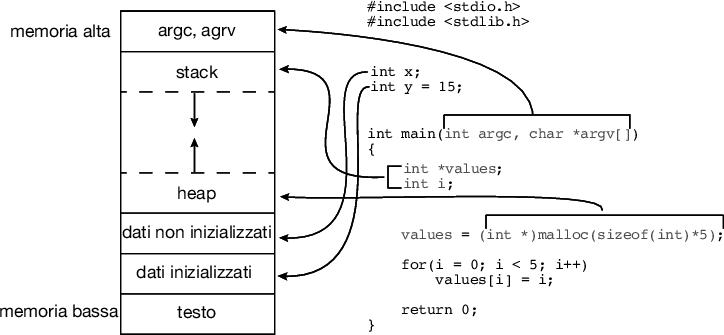
\includegraphics[width=0.5\linewidth]{images/Concetto-di-processo.png}
    \caption{Concetto di processo}
    \label{fig:prco1}
\end{figure}


     È anche corretto osservare che attraverso un programma si possono definire più processi, infatti:
    \begin{itemize}
        \item Lo stesso programma può contenere codice per generare più processi
        \item Più processi possono condividere lo stesso codice
    \end{itemize}
Tuttavia, la distinzione fondamentale tra processo e programma è che un processo \textbf{è un'entità attiva}, mentre un programma è \textbf{un'entità statica}.\\
\qs{}{Lo stesso programma lanciato due volte può dare origine a due processi diversi (perché?)}
Attenzione: processo, task, job sono \textbf{sinonimi}.\\

Un programma si \textbf{trasforma} in un processo quando viene lanciato, con il doppio click o da riga di comando.\\
Un processo può anche \textbf{nascere} a partire da un altro processo, quando quest’ultimo esegue una opportuna system call (fork, spawn, etc)\\

\dfn{Processo}{
In realtà, non sono due meccanismi distinti: un processo nasce sempre a partire da un altro processo, e sempre sotto il controllo e con l’intervento del SO (con un’unica eccezione, all’accensione del sistema).
}
\subsection{Stato del processo}
Da quanto nasce a quando termina, un processo passa la sua esistenza muovendosi tra un insieme di stati, e in ogni stante ogni processo si trova in un ben determinato stato. \\
Lo stato di un processo evolve a causa del codice eseguito e dell’azione del SO sui processi presenti nel sistema in un dato istante, secondo quanto illustrato dal diagramma di transizione degli stati di un processo.\\

\begin{figure}[h]
    \centering
    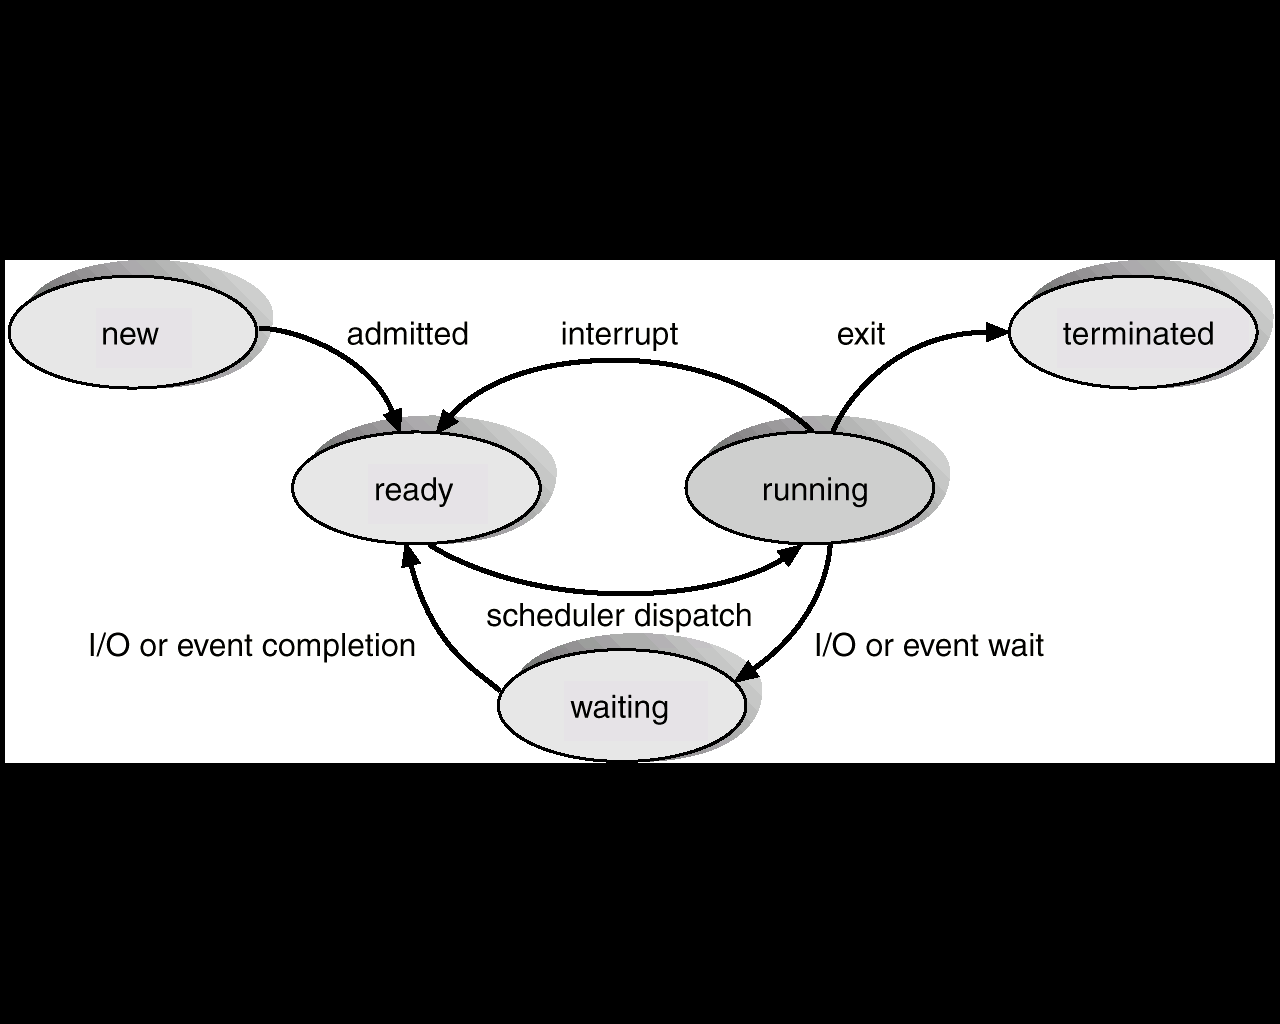
\includegraphics[width=0.5\linewidth]{images/StatoProcesso.png}
\end{figure}

\subsubsection{Gli stati}
Gli stati in cui può trovarsi un processo sono:
\dfn{Stati del processo}{\begin{itemize}
    \item \textbf{New}: Il processo è appena stato creato
    \item \textbf{Ready (to Run)}: Il processo è pronto per entrare in esecuzione
    \item \textbf{Running}: La CPU sta eseguendo il codice del processo
    \item \textbf{Waiting}: Il provesso ha lasciato la CPU e attende il completamento di un evento
    \item \textbf{Terminated}: Il processo è terminato, il SO sta recuperando le strutture dati e le aree di memoria liberate
\end{itemize}
}

Il diagramma di transizione degli stati di un processo sintetizza una serie di possibili varianti del modo in cui un sistema operativo (SO) può amministrare la vita dei processi di un computer.

\begin{itemize}
    \item Infatti, nel caso reale lo sviluppatore del SO dovrà decidere quali scelte implementative fare quando (ad esempio):
    \begin{itemize}
        \item Mentre il processo \(P_x\) è \textit{running}, un processo entra nello stato \textit{Ready to Run}
        \item Mentre il processo \(P_x\) è \textit{running}, un processo più importante di \(P_x\) entra nello stato \textit{Ready to Run}
        \item Mentre il processo \(P_x\) è nello stato \textit{Ready to Run}, un processo più importante di \(P_x\) entra nello stato \textit{Ready to Run}
    \end{itemize}
\end{itemize}

\qs{}{
Che significato ha eliminare l’arco “interrupt”?
}

Di avere un sistema non time-sharing

\subsection{Processo Control Block (PCB)}
Per ogni processo, il sistema operativo (SO) mantiene una struttura dati chiamata \textit{Process Control Block} (PCB), che contiene le informazioni necessarie per amministrare la vita di quel processo, tra cui:

\begin{itemize}
    \item Il numero del processo (o \textit{Process ID})(PID)
    \item Lo stato del processo (\textit{ready}, \textit{waiting},...)
    \item Il contenuto dei registri della CPU salvati nel momento in cui il processo è stato sospeso (valori significativi solo quando il processo non è \textit{running})
    \item Gli indirizzi in RAM delle aree dati e codice del processo
    \item I file e gli altri dispositivi di I/O correntemente in uso dal processo
    \item Le informazioni per lo \textit{scheduling} della CPU (ad esempio, quanta CPU ha usato fino a quel momento il processo)
\end{itemize}

\begin{figure}
    \centering
    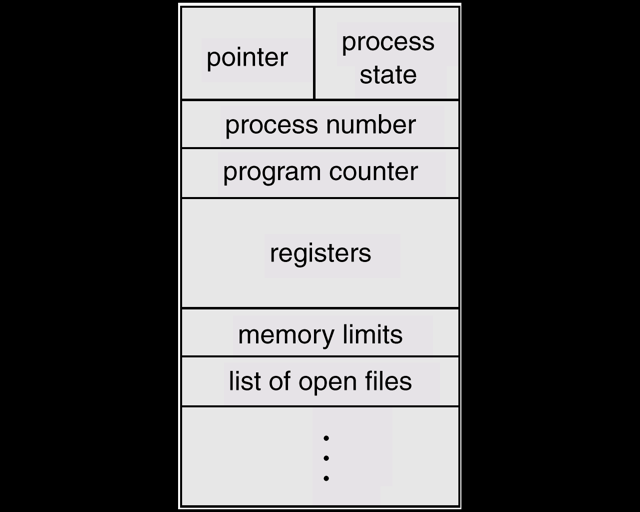
\includegraphics[width=0.5\linewidth]{images/Process-Control-Block.png}
\end{figure}

\section{Scheduling dei processi}
Conosciamo già i seguenti due concetti:

\begin{itemize}
    \item \textbf{Multiprogrammazione}: avere sempre un processo \textit{running} \(\Rightarrow\) massima utilizzazione della CPU.
    \item \textbf{Time Sharing}: distribuire l'uso della CPU fra i processi a intervalli prefissati. Così più utenti possono usare "allo stesso tempo" la macchina, e i loro processi procedono in "parallelo" (notate sempre le virgolette).
\end{itemize}

\dfn{Scheduling}{
Per implementare questi due concetti, il sistema operativo deve decidere periodicamente quale sarà il prossimo processo a cui assegnare la CPU. Questa operazione è detta \textit{Scheduling}.
}

In un sistema time sharing single-core, attraverso lo scheduling, ogni processo “crede” di avere a disposizione una macchina “tutta per se”...
Ci pensa il SO a farglielo credere, \textbf{commutando} la CPU fra i processi (ma succede la stessa cosa in un sistema ad n-core se ci sono più di n processi attivi contemporaneamente)
\begin{figure}[h]
    \centering
    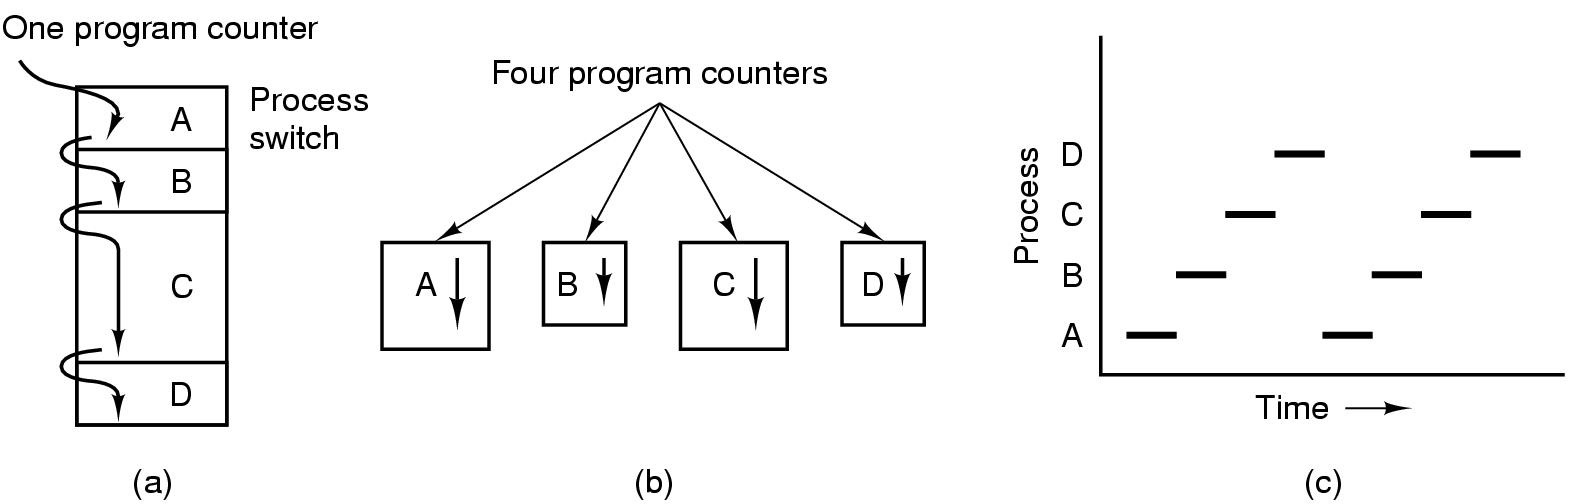
\includegraphics[width=0.5\linewidth]{images/SchedulingProcessi.png}
    \caption{a) Ciò che succede in realtà\\b) ciò che vede ogni singolo processo\\c) Il risultato finale}
\end{figure}

\subsection{Il cambio di contesto (context switch)}
Per commutare la CPU tra due processi, il sistema operativo deve:

\begin{enumerate}
    \item Riprendere il controllo della CPU (ad esempio attraverso il meccanismo del \textit{Timer} visto nel capitolo 1).
    \item Con l'aiuto dell'hardware della CPU, salvare lo stato corrente della computazione del processo che lascia la CPU, ossia copiare il valore del \textit{Program Counter} (PC) e degli altri registri nel suo \textit{Process Control Block} (PCB).
    \item Scrivere nel PC e nei registri della CPU i valori relativi contenuti nel PCB del processo utente scelto per entrare in esecuzione.
\end{enumerate}\\

Questa operazione prende il nome di: \textbf{cambio di contesto}, o \textit{context switch}.

Notate che, tecnicamente, anche il punto 1 è già di per sé un \textit{context switch}.

\begin{itemize}
    \item Il \textit{context switch} richiede tempo, perché il contesto di un processo è composto da molte informazioni (alcune le vedremo quando parleremo della gestione della memoria).
    \item Durante questa frazione di tempo, la CPU non è utilizzata da alcun processo utente.
    \item In generale, il \textit{context switch} può costare da qualche centinaio di nanosecondi a qualche microsecondo.
    \item Questo tempo “sprecato” rappresenta un \textit{overhead} (sovraccarico) per il sistema e influisce sulle sue prestazioni.
\end{itemize}

\begin{figure}[h]
    \centering
    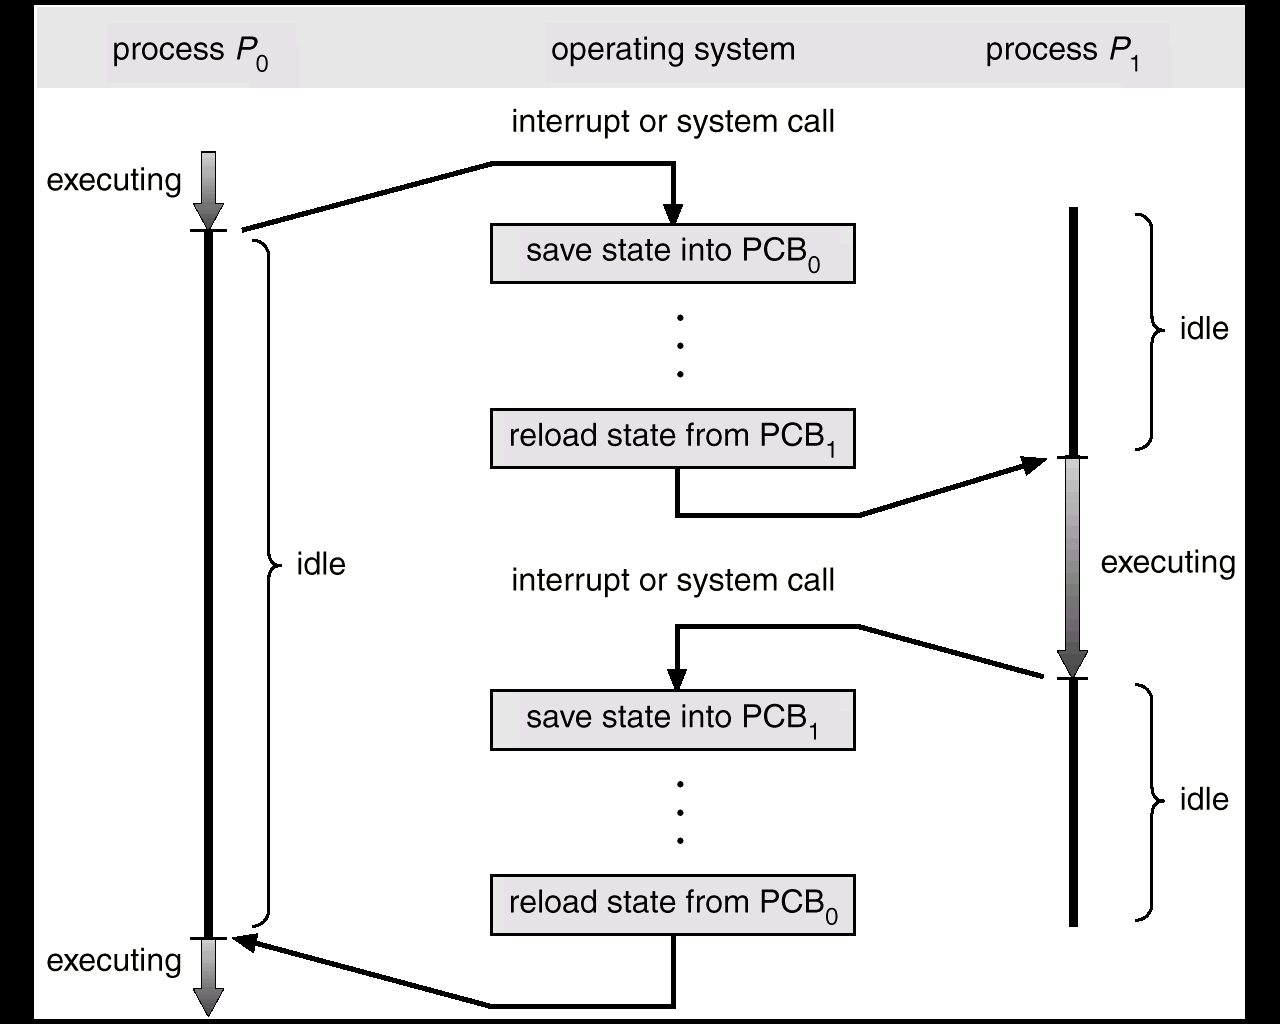
\includegraphics[width=0.5\linewidth]{images/Phases_of_scheduling.png}
    \caption{Fasi dello scheduling tra un processo e un altro}
\end{figure}

\subsection{Code di scheduling}
Per \textbf{amministrare} la vita di ciascun processo, il SO gestisce varie \textbf{code} di processi. Ogni processo “si trova” in una di queste code, a seconda di cosa sta facendo.
Una coda di processi non è altro che una lista di PCB, mantenuta in una delle aree di memoria primaria che il SO riserva a se stesso.\\
La coda dei processi più importante è la coda \textbf{ready}, o \textbf{ready queue (RQ)}: l'insieme dei processi \textbf{ready to run}.
\begin{figure}[h]
    \centering
    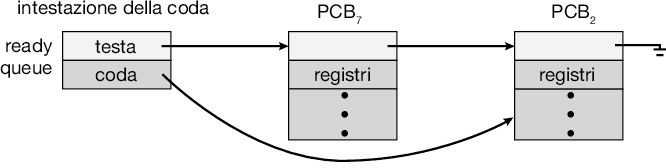
\includegraphics[width=0.5\linewidth]{images/ready_queue.png}
\end{figure}
Quando un processo rilascia la CPU, ma non termina e non torna nella \textit{ready queue}, vuol dire che si è messo in \textbf{attesa} di “qualcosa”, e il SO lo “parcheggia” in una tra le possibili code, che possiamo dividere in due grandi categorie:
\begin{itemize}
    \item \textbf{Device queues}: code dei processi in attesa per l’uso di un dispositivo di I/O. Una coda per ciascun dispositivo.
    \ex{Esempi}{
        \item Una coda d'attesa per il primo hard disk
        \item Una coda per l'ssd
        \item Una coda per la stampante, etc..
    }
    \item \textbf{Code di waiting}: code di processi in attesa che si verifichi un certo evento. Una coda per ciascun evento (ci torneremo nella sezione 6.6).
\end{itemize}
Dunque, durante la loro vita, i processi si spostano (meglio: il SO sposta i corrispondenti PCB) tra le varie code.\\
Quindi lo stato \textbf{waiting} nel diagramma di transizione degli stati di un processo \textbf{corrisponde a più code di attesa}

Possiamo riformulare il diagramma di transizione degli stati di un processo come un \textbf{diagramma di accodamento} in cui i processi si muovono fra le varie code 

\begin{figure}[h]
    \centering
    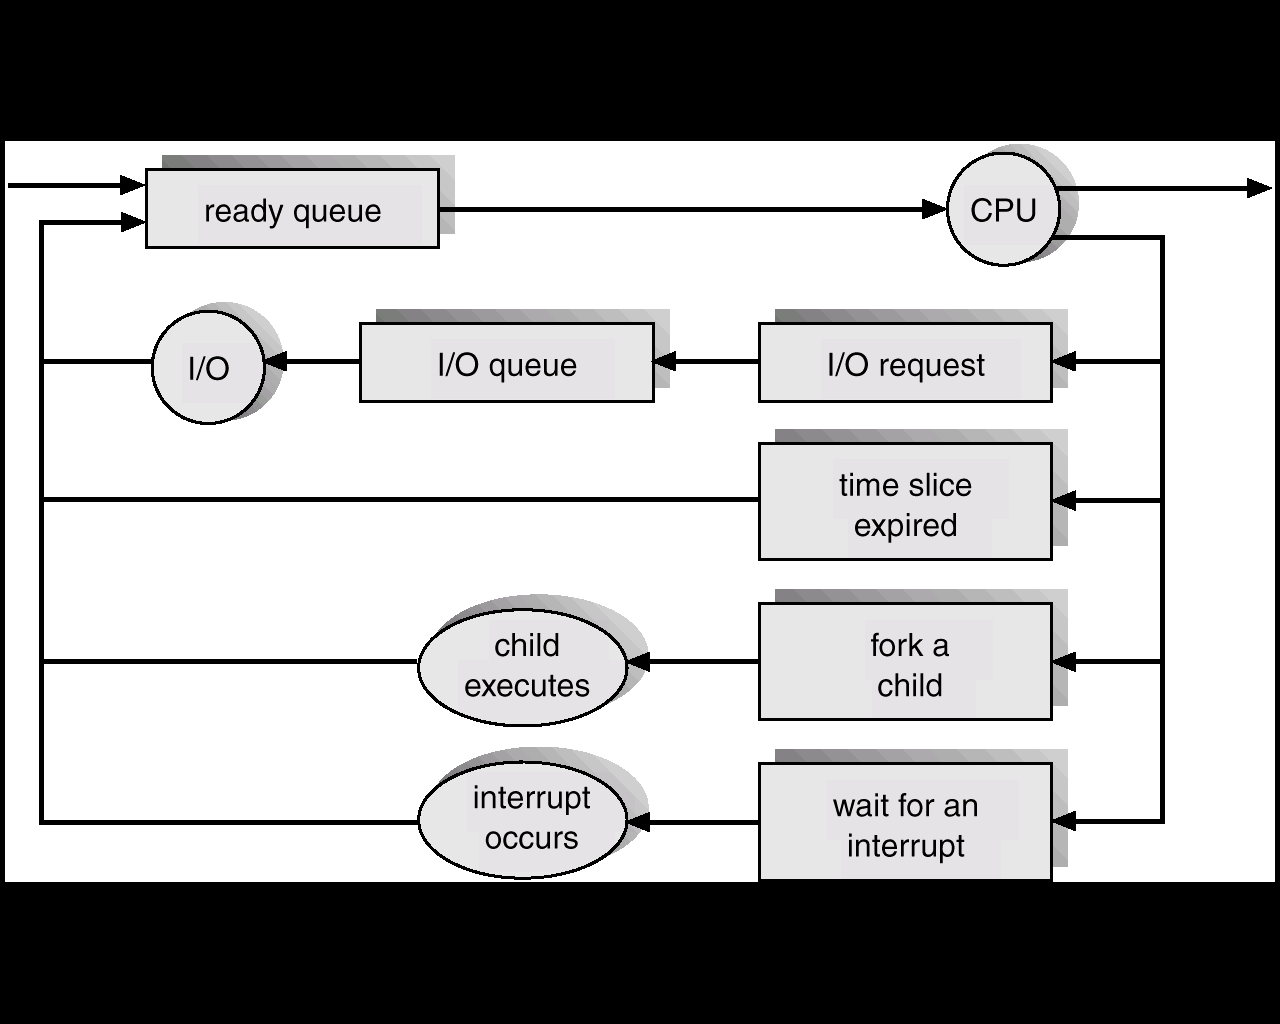
\includegraphics[width=0.5\linewidth]{images/Scheduling_queue_updated.png}
    \caption{SX: new, DX: Terminated}
\end{figure}

\subsection{CPU Scheduler}

Un componente del Sistema Operativo detto \textit{CPU Scheduler} sceglie uno dei processi nella coda \textit{ready} e lo manda in esecuzione.
\begin{itemize}
    \item Il \textit{CPU scheduler} si attiva ogni 50/100 millisecondi, ed è responsabile della realizzazione del \textit{time sharing}.
    \item Per limitare l'\textit{overhead}, deve essere molto veloce.
    \item Il \textit{CPU scheduler} è anche chiamato \textit{Short Term Scheduler}.
\end{itemize}


\section{Operazione sui processi}
La creazione di un processo è di gran lunga l’operazione più importante all’interno di qualsiasi sistema operativo.\\
Ogni SO possiede almeno una \textit{System Call} per la creazione di processi, e ogni processo è creato a partire da un altro processo usando la system call relativa (eccetto il processo che nasce all’accensione del sistema).\\
Il processo "creatore" è detto \textit{processo padre} (o \textit{parent}).\\
Il processo creato è detto \textit{processo figlio} (o \textit{child}).
\clm{}{}{
Poiché ogni processo può a sua volta creare altri processi, nel sistema si forma un “albero di processi”.}
\begin{figure}[h]
    \centering
    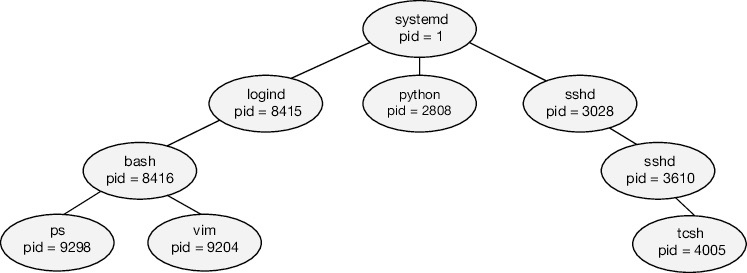
\includegraphics[width=0.5\linewidth]{images/Process_creation.png}
    \label{fig:creation_process}
\end{figure}

\subsection{Creazione di un processo}
Quando nasce un nuovo processo, il SO:
\begin{itemize}
    \item gli assegna un identificatore del processo unico, un numero intero detto \textbf{pid} (process-id). È il modo con cui il SO conosce e si riferisce a quel processo.
    \item recupera dall’hard disk il codice da eseguire e lo carica in RAM (a meno che il codice non sia già in RAM).
    \item alloca un nuovo \textit{PCB} e lo inizializza con le informazioni relative al nuovo processo.
    \item inserisce il \textit{PCB} in coda \textit{ready}.
\end{itemize}

\qs{}{Che cosa fa il processo padre quando ha generato un
processo figlio?}
\begin{itemize}
    \item Prosegue la sua esecuzione in modo concorrente all'esecuzione del processo figio, oppure:
    \item  Si ferma, in attesa del completamento dell'esecuzione del processo figlio
\end{itemize}
\qs{}{Quale codice esegue il processo figlio?}
\begin{itemize}
    \item al processo figlio viene data una copia del codice e dei dati in uso al processo padre, oppure:
    \item al processo figlio viene dato un nuovo programma, con eventualmente nuovi dati.
\end{itemize}

\subsection{Creazione di un processo in Unix}
\begin{lstlisting}[language=C]
int main() {
    /* fig. 3.8 modificata */
    pid_t pid, childpid;
    
    pid = fork(); /* genera un nuovo processo */
    printf("questa la stampano padre e figlio");
    
    if (pid == 0) { 
        /* processo figlio */
        printf("processo figlio");
        execlp("/bin/ls", "ls", NULL);
    } else {
        /* processo padre */
        printf("sono il padre, aspetto il figlio");
        childpid = wait(NULL);
        printf("il processo figlio è terminato");
        exit(0);
    }
}
\end{lstlisting}

\subsection{Passi dell'SO all'invocazione delle fork}
\begin{enumerate}
    \item Alloca un nuovo \textit{PCB} per il processo figlio e gli assegna un nuovo \textit{PID}; cerca un’area libera in RAM e vi copia le strutture dati e il codice del processo \textit{parent} (si veda più avanti): queste copie verranno usate dal processo figlio.
    \item Inizializza il \textit{PC} del figlio con l’indirizzo della prima istruzione successiva alla \textit{fork}.
    \item \textbf{Nella cella di memoria associata alla variabile che riceve il risultato della \textit{fork} del processo figlio scrive 0.}
    \item \textbf{Nella cella di memoria associata alla variabile che riceve il risultato della \textit{fork} del processo \textit{parent} scrive il \textit{PID} del figlio.}
    \item Mette i processi \textit{parent} e figlio in coda \textit{ready}.
\end{enumerate}

\clm{}{}{
$pid == 0$ Lo ha solo il processo figlio. \\
\textit{pid = id-child} LO ha solo il processo padre. \\
Così sono in grado di distinguere se sto operando con il figlio o con il padre
}

\subsubsection{Significato delle altre sys}
\textbf{Execlp}: Riceve in input un puntatore ad un file contenente codice eseguibile. Il processo che la invoca prosegue eseguendo il codice specificato, senza più ritornare alla porzione di codice che viene dopo la execlp.\\
\textbf{Wait}: Invocata da un processo parent, lo sospende fino alla terminazione del processo figlio. La wait restituisce il PID del figlio appena terminato.
\textbf{Exit:} provoca la terminazione istantanea del processo che la invoca.\\

\qs{}{Come cambia lo schema se il processo parent non esegue la wait?}
\begin{figure}[h]
    \centering
    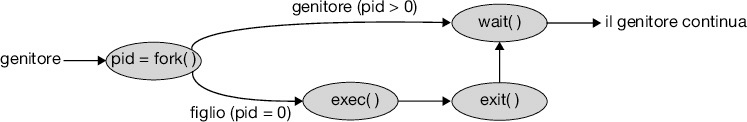
\includegraphics[width=0.5\linewidth]{images/child&parentLoveandFriend.png}
\end{figure}

\subsection{Altro esempio}
\begin{lstlisting}[language=C]
int main() {
    /* un altro esempio */
    int a, b, c = 57;
    a = fork(); // genera un nuovo processo
    printf("questa la stampano padre e figlio");
    
    if (a == 0) {
        /* processo figlio */
        c = 64; // ***
        printf("c = %d", c);
    } else {
        /* processo padre */
        printf("c = %d", c);
        b = wait(NULL);
        printf("b = %d", b);
    }
}
\end{lstlisting}
\subsection{Osservazioni}
\begin{itemize}
    \item Il codice viene condiviso tra padre e figlio, evitando duplicazione e spreco di memoria.
    \item Lo spazio dati viene duplicato: 
    \begin{itemize}
        \item Le modifiche di variabili non sono condivise tra padre e figlio.
        \item Le nuove variabili dichiarate dopo la \texttt{fork} non sono visibili all'altro processo.
    \end{itemize}
    \item Un padre può chiamare \texttt{fork} più volte, e usare il PID dei figli per tracciarli.
    \item \texttt{fork} restituisce 0 al figlio per distinguerlo dal padre.
    \item Se \texttt{fork} restituisse un valore maggiore di 0 al figlio, non si potrebbe distinguere facilmente tra padre e figlio, complicando la gestione delle operazioni diversificate (come illustrato in fig. 3.8).
\end{itemize}

\subsection{Terminazione di un processo}
Un processo termina dopo l'esecuzione dell'ultima istruzione del suo codice. Esiste una system call chiamata \texttt{exit()} per terminare un processo. \\
I dati di output, come il \texttt{pid}, possono essere inviati al processo padre in attesa della terminazione del figlio.
Il sistema operativo \textbf{rimuove} le risorse allocate al processo terminato, recuperando la RAM e chiudendo eventuali file aperti.

\begin{itemize}
    \item Un processo può uccidere esplicitamente un altro processo appartenente allo stesso utente tramite la system call \texttt{kill} (in Unix) o \texttt{TerminateProcess} (in Win32).
    \item In alcuni casi, il sistema operativo può decidere di terminare un processo utente, ad esempio se:
    \begin{itemize}
        \item il processo utilizza troppe risorse.
        \item il suo processo padre è morto (in questo caso può avvenire una terminazione a cascata, che non avviene però in Unix o Windows).
    \end{itemize}
\end{itemize}

\section{Comunicazione tra processi}
\textbf{Processi indipendenti e cooperanti}

I processi attivi in un sistema possono essere classificati come:

\begin{itemize}
    \item \textbf{Indipendenti}: quando non si influenzano esplicitamente durante l'esecuzione.
    \item \textbf{Cooperanti}: quando si influenzano a vicenda per:
    \begin{itemize}
        \item Scambiarsi informazioni.
        \item Collaborare su un'elaborazione suddivisa per efficienza o modularità.
    \end{itemize}
\end{itemize}

I processi cooperanti necessitano di meccanismi di comunicazione e sincronizzazione.

\section{Esempio: il problema Produttore-Consumatore}
\textbf{Problema del produttore-consumatore}

Un classico problema di processi cooperanti è il \textit{problema del produttore-consumatore}:

\begin{itemize}
    \item Un \textbf{processo produttore} produce informazioni che vengono consumate da un \textbf{processo consumatore}.
    \item Le informazioni sono collocate in un buffer di dimensione limitata.
    \item Un esempio pratico è un \textbf{processo compilatore} (produttore) che genera codice assembler.
    \item Il \textbf{processo assemblatore} (consumatore) traduce il codice assembler in linguaggio macchina.
    \item L'assemblatore potrebbe poi diventare un produttore per un modulo che carica in RAM il codice.
\end{itemize}

\begin{lstlisting}[language=C]
#define SIZE 10

typedef struct {
    // Definizione della struttura dell'item
    ...
} item;

// Buffer condiviso
item buffer[SIZE]; (shared array)

// Variabili condivise
int in = 0, out = 0; 
\end{lstlisting}

\textbf{Buffer circolare} di \texttt{SIZE} elementi con due puntatori \texttt{in} e \texttt{out}:
\begin{itemize}
    \item \texttt{in}: indica la prossima posizione libera nel buffer.
    \item \texttt{out}: indica la prossima posizione piena da consumare.
    \item \textbf{Condizione di buffer vuoto}: \texttt{in == out}.
    \item \textbf{Condizione di buffer pieno}: \texttt{(in + 1) \% SIZE == out}.
\end{itemize}

\textit{Nota}: la soluzione utilizza solo \texttt{SIZE-1} elementi per evitare conflitti tra la condizione di buffer pieno e vuoto.

